\documentclass[12pt, border=1pt, multi, tikz]{standalone}
%\usepackage{blocks}
\usepackage{xcolor}
\usepackage{import}
\subimport{../../layers/}{init}
\usetikzlibrary{positioning}
\usetikzlibrary{3d}

\def\ConvColor{rgb:yellow,5;red,2.5;white,5}
\def\ConvReluColor{rgb:yellow,5;red,5;white,5}

\def\PoolColor{rgb:red,1;black,0.3}
\def\UnpoolColor{rgb:blue,2;green,1;black,0.3}

\def\FcColor{rgb:blue,5;red,2.5;white,5}
\def\FcReluColor{rgb:blue,5;red,5;white,4}
\def\SoftmaxColor{rgb:magenta,5;black,7}

\def\TC{black}

\color{\TC}


\newcommand{\copymidarrow}{\tikz \draw[-Stealth,line width =0.8mm,draw={rgb:blue,4;red,1;green,1;black,3}] (-0.3,0) -- ++(0.3,0);}

\begin{document}
\begin{tikzpicture}
\tikzstyle{connection}=[ultra thick,every node/.style={sloped,allow upside down},draw=\edgecolor,opacity=0.3]
\tikzstyle{copyconnection}=[ultra thick,every node/.style={sloped,allow upside down},draw={rgb:blue,4;red,1;green,1;black,3},opacity=0.6]


% Input
\node[canvas is zy plane at x=0] (temp) at (-1,0,0) 
        {
        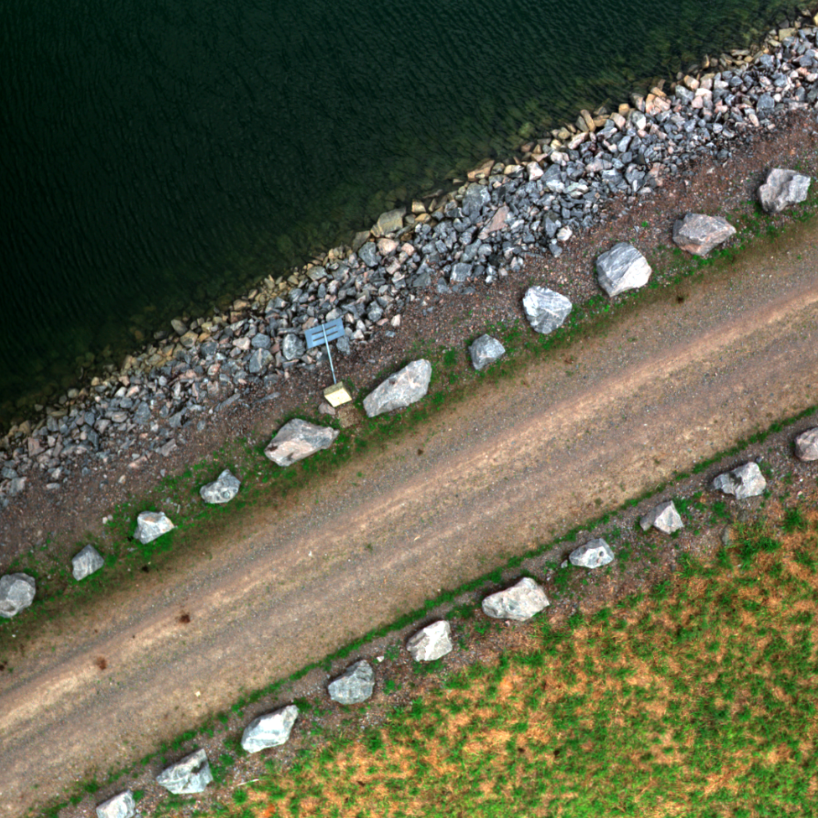
\includegraphics[width=8cm,height=8cm]{input.png},
        };


% Encoder
% conv2d + conv2d_1
\pic[shift={ (0,0,0) }] at (0,0,0) 
    {RightBandedBox={
        name=conv0-1,
        caption= ,
        xlabel={{ 16, 16 }},
        zlabel=\\256x256,
        fill=\ConvColor,
        bandfill=\ConvReluColor,
        height=40,
        width={ 2 , 2 },
        depth=40
        }
    };

% max_pooling2d
\pic[shift={ (0,0,0) }] at (conv0-1-east) 
    {Box={
        name=pool_0,
        caption= ,
        fill=\PoolColor,
        opacity=0.5,
        height=32,
        width=1,
        depth=32
        }
    };

% conv2d_2 + conv2d_3
\pic[shift={ (0.5,-1.1,0) }] at (pool_0-east) 
    {RightBandedBox={
        name=conv2-3,
        caption= ,
        xlabel={{ 32, 32 }},
        zlabel=\\128x128,
        fill=\ConvColor,
        bandfill=\ConvReluColor,
        height=32,
        width={ 2.8 , 2.8 },
        depth=32
        }
    };

% max_pooling2d_1
\pic[shift={ (0,0,0) }] at (conv2-3-east) 
{Box={
    name=pool_1,
    caption= ,
    fill=\PoolColor,
    opacity=0.5,
    height=24,
    width=1,
    depth=24
    }
};

% conv2d_4 + conv2d_5
\pic[shift={ (0.5,-1.1,0) }] at (pool_1-east) 
    {RightBandedBox={
        name=conv4-5,
        caption= ,
        xlabel={{ 64, 64 }},
        zlabel=\\64x64,
        fill=\ConvColor,
        bandfill=\ConvReluColor,
        height=24,
        width={ 3.6 , 3.6 },
        depth=24
        }
    };

% max_pooling2d_2
\pic[shift={ (0,0,0) }] at (conv4-5-east) 
{Box={
    name=pool_2,
    caption= ,
    fill=\PoolColor,
    opacity=0.5,
    height=16,
    width=1,
    depth=16
    }
};

% conv2d_6 + conv2d_7
\pic[shift={ (0.5,-1.1,0) }] at (pool_2-east) 
    {RightBandedBox={
        name=conv6-7,
        caption= ,
        xlabel={{ 128, 128 }},
        zlabel=\\32x32,
        fill=\ConvColor,
        bandfill=\ConvReluColor,
        height=16,
        width={ 4.4 , 4.4 },
        depth=16
        }
    };

% max_pooling2d_3
\pic[shift={ (0,0,0) }] at (conv6-7-east) 
{Box={
    name=pool_3,
    caption= ,
    fill=\PoolColor,
    opacity=0.5,
    height=8,
    width=1,
    depth=8
    }
};

% Bottleneck
% conv2d_8 + conv2d_9
\pic[shift={ (0.5,-1.1,0) }] at (pool_3-east) 
    {RightBandedBox={
        name=conv8-9,
        caption= ,
        xlabel={{ 256, 256 }},
        zlabel=\\16x16,
        fill=\ConvColor,
        bandfill=\ConvReluColor,
        height=8,
        width={ 5.2 , 5.2 },
        depth=8
        }
};

% Decoder
% Unpool 0
\pic[shift={ (1.2,+1.1,0) }] at (conv8-9-east) 
{Box={
    name=unpool_0,
    caption= ,
    fill=\UnpoolColor,
    opacity=0.5,
    height=16,
    width=1,
    depth=16
    }
};

% conv2d_transpose
\pic[shift={ (0,0,0) }] at (unpool_0-east) 
    {RightBandedBox={
        name=convt_0,
        caption= ,
        xlabel={ 128, "" },
        % zlabel=\\16x16,
        fill=\ConvColor,
        bandfill=\ConvReluColor,
        height=16,
        width={ 4.4 },
        depth=16
        }
};

% cat
\pic[shift={ (0,0,0) }] at (convt_0-east) 
    {RightBandedBox={
        name=cat_4,
        xlabel={{ 128, "" }},
        fill={rgb:white,1;black,3},
        bandfill={rgb:white,1;black,2},
        opacity=0.2,
        height=16,
        width={4.4},
        depth=16
        }
};

% conv2d_transpose + conv2d_10
\pic[shift={ (0,0,0) }] at (cat_4-east) 
    {RightBandedBox={
        name=conv10_11,
        caption= ,
        xlabel={{ 128, 128 }},
        zlabel=\\32x32,
        fill=\ConvColor,
        bandfill=\ConvReluColor,
        height=16,
        width={ 4.4 , 4.4 },
        depth=16
        }
};

% Unpool 1
\pic[shift={ (1.2,+1.1,0) }] at (conv10_11-east) 
{Box={
    name=unpool_1,
    caption= ,
    fill=\UnpoolColor,
    opacity=0.5,
    height=24,
    width=1,
    depth=24
    }
};

% conv2d_transpose
\pic[shift={ (0,0,0) }] at (unpool_1-east) 
    {RightBandedBox={
        name=convt_1,
        caption= ,
        xlabel={ 64, "" },
        % zlabel=\\16x16,
        fill=\ConvColor,
        bandfill=\ConvReluColor,
        height=24,
        width={ 3.6 },
        depth=24
        }
};

% cat
\pic[shift={ (0,0,0) }] at (convt_1-east) 
    {RightBandedBox={
        name=cat_3,
        xlabel={{ 64, "" }},
        fill={rgb:white,1;black,3},
        bandfill={rgb:white,1;black,2},
        opacity=0.2,
        height=24,
        width={3.6},
        depth=24
        }
};

% conv2d_12 + conv2d_13
\pic[shift={ (0,0,0) }] at (cat_3-east) 
    {RightBandedBox={
        name=conv12_13,
        caption= ,
        xlabel={{ 64, 64 }},
        zlabel=\\64x64,
        fill=\ConvColor,
        bandfill=\ConvReluColor,
        height=24,
        width={ 3.6 , 3.6 },
        depth=24
        }
};

% Unpool 1
\pic[shift={ (1.2,+1.1,0) }] at (conv12_13-east) 
{Box={
    name=unpool_2,
    caption= ,
    fill=\UnpoolColor,
    opacity=0.5,
    height=32,
    width=1,
    depth=32
    }
};

% conv2d_transpose
\pic[shift={ (0,0,0) }] at (unpool_2-east) 
    {RightBandedBox={
        name=convt_2,
        caption= ,
        xlabel={ 32, "" },
        % zlabel=\\16x16,
        fill=\ConvColor,
        bandfill=\ConvReluColor,
        height=32,
        width={ 2.8 },
        depth=32
        }
};

% cat
\pic[shift={ (0,0,0) }] at (convt_2-east) 
    {RightBandedBox={
        name=cat_2,
        xlabel={{ 32, "" }},
        fill={rgb:white,1;black,3},
        bandfill={rgb:white,1;black,2},
        opacity=0.2,
        height=32,
        width={2.8},
        depth=32
        }
};

% conv2d_14 + conv2d_15
\pic[shift={ (0,0,0) }] at (cat_2-east) 
    {RightBandedBox={
        name=conv14_15,
        caption= ,
        xlabel={{ 32, 32 }},
        zlabel=\\128x128,
        fill=\ConvColor,
        bandfill=\ConvReluColor,
        height=32,
        width={ 2.8 , 2.8 },
        depth=32
        }
};

% Unpool 3
\pic[shift={ (1.3,+1.1,0) }] at (conv14_15-east) 
{Box={
    name=unpool_3,
    caption= ,
    fill=\UnpoolColor,
    opacity=0.5,
    height=40,
    width=1,
    depth=40
    }
};

% conv2d_transpose
\pic[shift={ (0,0,0) }] at (unpool_3-east) 
    {RightBandedBox={
        name=convt_3,
        caption= ,
        xlabel={ 16, "" },
        % zlabel=\\16x16,
        fill=\ConvColor,
        bandfill=\ConvReluColor,
        height=40,
        width={ 2 },
        depth=40
        }
};

% cat
\pic[shift={ (0,0,0) }] at (convt_3-east) 
    {RightBandedBox={
        name=cat_1,
        xlabel={{ 16, "" }},
        fill={rgb:white,1;black,3},
        bandfill={rgb:white,1;black,2},
        opacity=0.2,
        height=40,
        width={2},
        depth=40
        }
};

% conv2d_16 + conv2d_17
\pic[shift={ (0,0,0) }] at (cat_1-east) 
    {RightBandedBox={
        name=conv17_18,
        caption= ,
        xlabel={{ 16, 16 }},
        % zlabel=\\256x256,
        fill=\ConvColor,
        bandfill=\ConvReluColor,
        height=40,
        width={ 2 , 2 },
        depth=40
        }
};

%
\pic[shift={(0.75,0,0)}] at (conv17_18-east)
        {Box={
                name=output,
                % caption=\\Softmax,
                zlabel=\\256x256,
                fill=\SoftmaxColor,
                height=40,
                width=1,
                depth=40}};


% Output
\node[canvas is zy plane at x=0.3] (temp) at (output-east) 
        {
        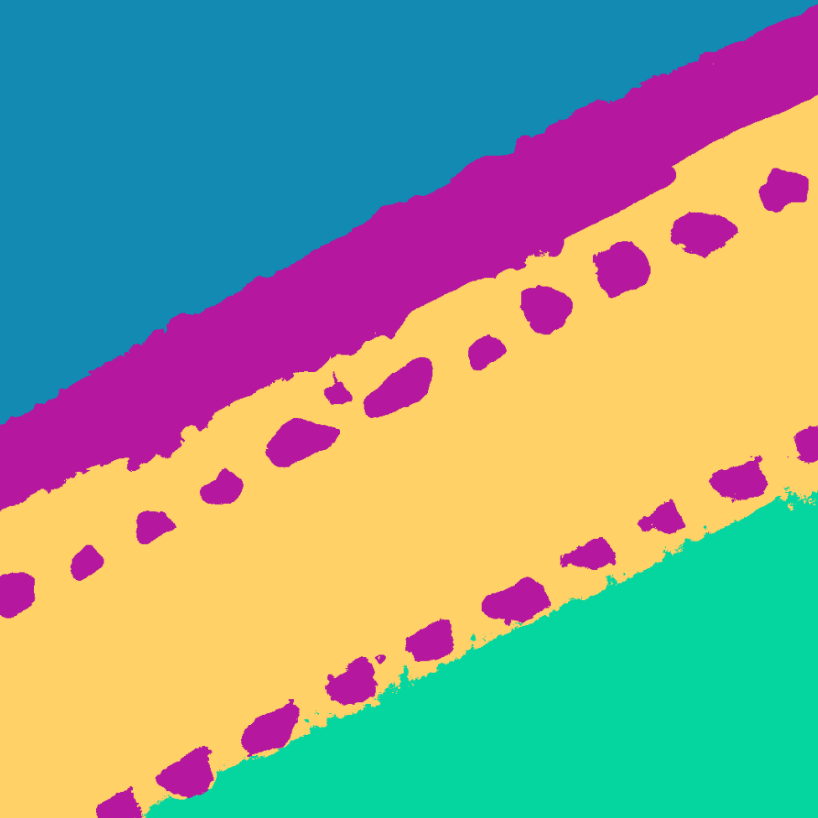
\includegraphics[width=8cm,height=8cm]{output.png},
        };



% Conections

% Encoder
\draw [connection]  (pool_0-east)    -- node {\midarrow} (conv2-3-west);
\draw [connection]  (pool_1-east)    -- node {\midarrow} (conv4-5-west);
\draw [connection]  (pool_2-east)    -- node {\midarrow} (conv6-7-west);
\draw [connection]  (pool_3-east)    -- node {\midarrow} (conv8-9-west);

% Decoder
\draw [connection]  (conv8-9-east)    -- node {\midarrow} (unpool_0-west);
\draw [connection]  (conv10_11-east)    -- node {\midarrow} (unpool_1-west);
\draw [connection]  (conv12_13-east)    -- node {\midarrow} (unpool_2-west);
\draw [connection]  (conv14_15-east)    -- node {\midarrow} (unpool_3-west);
\draw [connection]  (conv17_18-east)    -- node {\midarrow} (output-west);

% Skip Paths
\path (conv6-7-southeast) -- (conv6-7-northeast) coordinate[pos=1.25] (conv6-7-top);
\path (cat_4-south)  -- (cat_4-north)  coordinate[pos=1.25] (cat_4-top);

\path (conv4-5-southeast) -- (conv4-5-northeast) coordinate[pos=1.25] (conv4-5-top);
\path (cat_3-south)  -- (cat_3-north)  coordinate[pos=1.25] (cat_3-top);

\path (conv2-3-southeast) -- (conv2-3-northeast) coordinate[pos=1.25] (conv2-3-top);
\path (cat_2-south)  -- (cat_2-north)  coordinate[pos=1.25] (cat_2-top);

\path (conv0-1-southeast) -- (conv0-1-northeast) coordinate[pos=1.25] (conv0-1-top);
\path (cat_1-south)  -- (cat_1-north)  coordinate[pos=1.25] (cat_1-top);

% Skip Connections
\draw [copyconnection]  (conv6-7-northeast)  
-- node {\copymidarrow}(conv6-7-top)
-- node {\copymidarrow}(cat_4-top)
-- node {\copymidarrow} (cat_4-north);

\draw [copyconnection]  (conv4-5-northeast)  
-- node {\copymidarrow}(conv4-5-top)
-- node {\copymidarrow}(cat_3-top)
-- node {\copymidarrow} (cat_3-north);

\draw [copyconnection]  (conv2-3-northeast)  
-- node {\copymidarrow}(conv2-3-top)
-- node {\copymidarrow}(cat_2-top)
-- node {\copymidarrow} (cat_2-north);

\draw [copyconnection]  (conv0-1-northeast)  
-- node {\copymidarrow}(conv0-1-top)
-- node {\copymidarrow}(cat_1-top)
-- node {\copymidarrow} (cat_1-north);


% Legend
\pic[shift={ (0,0,0) }] at (0,-8,0) 
    {RightBandedBox={
        name=conv-legend,
        caption= \textcolor{\TC}{\large{Convolução + \\ ReLU}},
        % xlabel={{ 16, 16 }},
        % zlabel=\\256x256,
        fill=\ConvColor,
        bandfill=\ConvReluColor,
        height=5,
        width={ 5 },
        depth=5
        }
    };

\pic[shift={ (+5,0,0) }] at (conv-legend-east) 
    {Box={
        name=pool-legend,
        caption=\textcolor{\TC}{\large{MaxPooling}},
        fill=\PoolColor,
        opacity=0.5,
        height=5,
        width=5,
        depth=5
        }
    };

\pic[shift={ (+5,0,0) }] at (pool-legend-east) 
   {Box={
        name=unpool-legend,
        caption=\textcolor{\TC}{\large{MaxUnpooling}},
        fill=\UnpoolColor,
        opacity=0.5,
        height=5,
        width=5,
        depth=5
        }
};

\pic[shift={ (+5,0,0) }] at (unpool-legend-east) 
    {RightBandedBox={
        name=cat-legend,
        caption=\textcolor{\TC}{\large{Concatenação}},
        fill={rgb:white,1;black,3},
        bandfill={rgb:white,1;black,2},
        opacity=0.2,
        height=5,
        width=5,
        depth=5
        }
};

\pic[shift={(+5,0,0)}] at (cat-legend-east)
        {Box={
                name=output-legend,
                caption=\textcolor{\TC}{\large{Convolução + Sigmóide}},
                fill=\SoftmaxColor,
                height=5,
                width=5,
                depth=5}
                };


\end{tikzpicture}
\end{document}